% hmesh.tex: libhmesh as it is in main, with the plans to come.
% Build with make (two pdflatex passes); the PDF is not kept in git.
\documentclass[10pt,a4paper]{article}
\usepackage[margin=2cm]{geometry}
\usepackage[T1]{fontenc}
\usepackage{lmodern}
\usepackage{amsmath}
\usepackage{amssymb}
\usepackage{amsthm}
\usepackage{booktabs}
\usepackage{array}
\usepackage{tabularx}
\usepackage{xcolor}
\usepackage{tikz}
\usetikzlibrary{arrows.meta, calc, decorations.markings}
\usepackage{float}
\usepackage{algorithm}
\usepackage{algpseudocode}
\algrenewcommand\algorithmicrequire{\textbf{In:}}
\algrenewcommand\algorithmicensure{\textbf{Out:}}
\algrenewcommand\algorithmiccomment[1]{\hfill{\footnotesize\color{black!60}\(\triangleright\) #1}}
\usepackage{caption}
\usepackage[hidelinks]{hyperref}
\usepackage{enumitem}
\setlist{nosep, leftmargin=1.4em}
\captionsetup{font=small, labelfont=bf}
\setlength{\parindent}{0pt}
\setlength{\parskip}{0.55em}
\theoremstyle{definition}
\newtheorem{definition}{Definition}
\newtheorem{proposition}{Proposition}

% Okabe-Ito colours, safe for colour blindness
\definecolor{c0}{HTML}{0072B2}
\definecolor{c1}{HTML}{E69F00}
\definecolor{c2}{HTML}{009E73}
\definecolor{c3}{HTML}{CC79A7}

\newcommand{\fn}[1]{\texttt{#1}}
\newcommand{\twin}{\operatorname{twin}}
\newcommand{\nxt}{\operatorname{next}}

\tikzset{
  half/.style={-{Stealth[length=4pt]}, line width=0.7pt},
  pt/.style={circle, fill=black, inner sep=1.2pt},
}

\title{libhmesh\\[2pt]
  \large a simplicial manifold in a block-AMR tree}
\author{libhmesh notes}
\date{}

\begin{document}
\maketitle

\noindent
libhmesh holds a simplicial manifold of dimension $m$ in $\mathbb{R}^D$,
$0 \le m \le D \le 3$: points, a curve (a river network), a surface (an
interface between water and air), a volume. It is a half-edge mesh
generalised to every level of the complex, with fields on every level. It
lives inside libb-amr's block-structured tree: its points are sorted along
the tree's Morton curve, it gives the tree's cells their volume fractions
exactly, and it is moved by the tree's face velocities. This note describes
the library as it is in main; the last section lists what is planned.

\tableofcontents

% ======================================================================
\section{The model}
\label{sec:model}

\subsection{Levels}

A mesh of dimension $m$ has levels $k = 0, \ldots, m$. Level $k$ holds the
$k$-simplices. Every face of every simplex is stored once, at its own
level, with its own id: a triangle's three edges are level 1 simplices, and
its three points level 0 ones. So each level carries its own fields: depths
on triangles, fluxes on edges, heights on points. A simplex at level $k$ is
a list of $k + 1$ point ids $s = (v_0, \ldots, v_k)$, which also gives its
orientation.

\subsection{Halves}

\begin{definition}[halves]
  A $k$-simplex $s = (v_0, \ldots, v_k)$, $k \ge 1$, has $k + 1$ halves,
  numbered $h = (k + 1)\,s + i$, $0 \le i \le k$. Half $i$ stands for the
  facet opposite $v_i$, that is $(v_0, \ldots, \widehat{v_i}, \ldots,
  v_k)$. Each half has:
  \begin{itemize}
    \item its vertex $v_i$, the one opposite its facet (\fn{hm\_half\_vertex});
    \item its facet's id at level $k - 1$ (\fn{hm\_half\_facet});
    \item its sign, the incidence number: $+1$ if the orientation $s$
      induces on the facet, $(-1)^i (v_0 \ldots \widehat{v_i} \ldots
      v_k)$, is the facet's own, else $-1$ (\fn{hm\_half\_sign});
    \item $\nxt(h)$: half $i + 1 \bmod k + 1$ of the same simplex, computed,
      not stored (\fn{hm\_half\_next});
    \item $\twin(h)$: the next half, of another $k$-simplex, on the same
      facet (\fn{hm\_half\_twin}).
  \end{itemize}
\end{definition}

\begin{center}
\begin{tabular}{@{}cll@{}}
  \toprule
  $k$ & halves & the twin cycle turns about \\
  \midrule
  1 & 2 half-points (an edge's ends) & a point: the edges at it \\
  2 & 3 half-edges & an edge: the triangles on it \\
  3 & 4 half-faces & a triangle: the tetrahedra on it \\
  \bottomrule
\end{tabular}
\end{center}

For a triangle the halves are those of a half-edge mesh: half $i$ goes
from $v_{i+1}$ to $v_{i+2}$ (\fn{hm\_half\_origin}), and
$\twin(\nxt(\nxt(h)))$ turns about the origin of $h$
(figure~\ref{fig:halves}).

\begin{figure}[H]
\centering
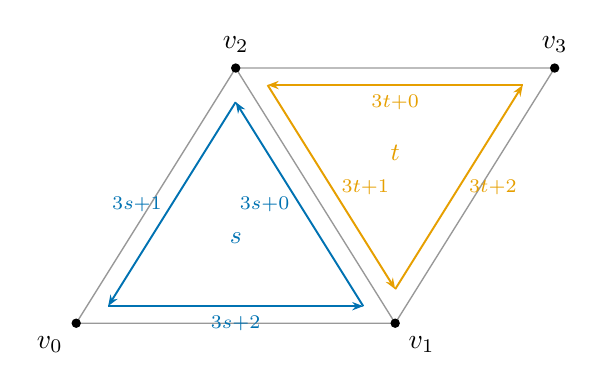
\begin{tikzpicture}[scale=1.35]
  \coordinate (v0) at (0,0);
  \coordinate (v1) at (3,0);
  \coordinate (v2) at (1.5,2.4);
  \coordinate (v3) at (4.5,2.4);
  \coordinate (gs) at ($1/3*(v0)+1/3*(v1)+1/3*(v2)$);
  \coordinate (gt) at ($1/3*(v1)+1/3*(v3)+1/3*(v2)$);
  \draw[black!40, line width=0.5pt] (v0) -- (v1) -- (v2) -- cycle;
  \draw[black!40, line width=0.5pt] (v1) -- (v3) -- (v2);
  % halves of s = (v0, v1, v2): half i from v(i+1) to v(i+2)
  \draw[half, c0] ($(v1)!0.2!(gs)$) -- ($(v2)!0.2!(gs)$)
    node[midway, left, font=\scriptsize] {$3s{+}0$};
  \draw[half, c0] ($(v2)!0.2!(gs)$) -- ($(v0)!0.2!(gs)$)
    node[midway, left, font=\scriptsize] {$3s{+}1$};
  \draw[half, c0] ($(v0)!0.2!(gs)$) -- ($(v1)!0.2!(gs)$)
    node[midway, below, font=\scriptsize] {$3s{+}2$};
  % halves of t = (v1, v3, v2)
  \draw[half, c1] ($(v3)!0.2!(gt)$) -- ($(v2)!0.2!(gt)$)
    node[midway, below, font=\scriptsize] {$3t{+}0$};
  \draw[half, c1] ($(v2)!0.2!(gt)$) -- ($(v1)!0.2!(gt)$)
    node[midway, right, font=\scriptsize] {$3t{+}1$};
  \draw[half, c1] ($(v1)!0.2!(gt)$) -- ($(v3)!0.2!(gt)$)
    node[midway, right, font=\scriptsize] {$3t{+}2$};
  \foreach \p/\a/\l in {v0/below left/v_0, v1/below right/v_1,
      v2/above/v_2, v3/above/v_3}
    \node[pt, label=\a:{$\l$}] at (\p) {};
  \node[c0, font=\small] at (gs) {$s$};
  \node[c1, font=\small] at (gt) {$t$};
\end{tikzpicture}
\caption{Two triangles $s = (v_0, v_1, v_2)$ and $t = (v_1, v_3, v_2)$,
  both counterclockwise. Half $i$ of a triangle is the edge opposite
  $v_i$, drawn from $v_{i+1}$ to $v_{i+2}$. The shared edge $v_1 v_2$ is
  one level 1 simplex; its two halves $3s{+}0$ and $3t{+}1$ are twins, of
  opposite signs.}
\label{fig:halves}
\end{figure}

\subsection{Twins are cycles}

The halves on one facet form a cycle under $\twin$, whatever their number:
\begin{itemize}
  \item inside the manifold, at level $m$, a facet has two halves and
    $\twin$ is an involution: $\twin(\twin(h)) = h$, the neighbour across,
    of the opposite sign when the orientation is consistent;
  \item on a boundary the cycle is $h$ alone (\fn{hm\_half\_boundary});
  \item at a junction, as at a confluence of three river branches, the
    cycle holds them all (figure~\ref{fig:junction}), so a junction needs no
    special case;
  \item below level $m$ a cycle holds every coface, in no particular order:
    the edges at a point of a surface.
\end{itemize}

\begin{figure}[H]
\centering
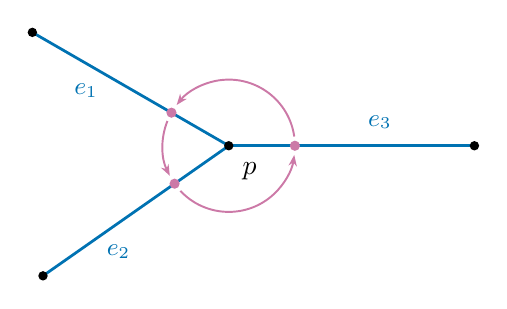
\begin{tikzpicture}[scale=1.2]
  \coordinate (p) at (0,0);
  % the three edges, at 150, 215 and 0 degrees from p
  \foreach \ang/\len/\l in {150/2.4/e_1, 215/2.4/e_2, 0/2.6/e_3} {
    \draw[c0, line width=1pt] (p) -- (\ang:\len);
    \node[pt] at (\ang:\len) {};
    \node[c0, font=\small] at ($(\ang:1.6) + (\ang+90:0.25)$) {$\l$};
    \node[circle, fill=c3, inner sep=1.3pt] at (\ang:0.7) {};
  }
  % twin: e1's half at p -> e2's -> e3's -> e1's
  \draw[half, c3] (158:0.7) arc[start angle=158, end angle=207, radius=0.7];
  \draw[half, c3] (223:0.7) arc[start angle=223, end angle=352, radius=0.7];
  \draw[half, c3] (8:0.7) arc[start angle=8, end angle=142, radius=0.7];
  \node[pt, label={[label distance=1pt]-60:{$p$}}] at (p) {};
\end{tikzpicture}
\caption{A confluence: three edges of a curve meet at the point $p$. Each
  edge has a half whose facet is $p$ (the dots); the three form one $\twin$
  cycle, $e_1 \to e_2 \to e_3 \to e_1$.
  The point's use (\fn{hm\_use}) is one of them, the entry into the
  cycle.}
\label{fig:junction}
\end{figure}

\subsection{Uses and signs}

A $(k-1)$-simplex keeps one half on it at level $k$, its use
(\fn{hm\_use}): the entry into its cycle. \fn{hm\_use (M, 0, v)} starts the
walk through the edges at the point $v$.

The signs are the boundary operator: $\partial (v_0, v_1) = v_1 - v_0$, and
in general
\[
  \partial (v_0, \ldots, v_k) = \sum_{i=0}^{k} (-1)^i\, (v_0, \ldots,
    \widehat{v_i}, \ldots, v_k),
\]
each term written as $\pm$ the facet as it is stored. Then $\partial
\partial = 0$ at every level, which the tests check. A flux on an edge,
added to a triangle with \fn{hm\_half\_sign}, is a conservative divergence
whatever the orientation of the edges.

% ======================================================================
\section{Storage}
\label{sec:storage}

Per level, a structure of arrays: the halves' vertices, twins and facets at
index $(k + 1)\,s + i$ (the facet's sign in its top bit), one use per
simplex below the top level, the points' coordinates $x_0, x_1, x_2$ as
three arrays, and each component of each field as an array of its own. Ids
are 32 bit; \fn{HM\_NONE} ($2^{32} - 1$) is no simplex, no half.

\begin{itemize}
  \item \textbf{Push.} An id from the stack of freed ids, the last freed
    first (its memory is still in cache), else the end of the arrays, which
    double as they fill. A new simplex's field values are zero.
  \item \textbf{Remove, anywhere.} Its bit in the alive bitmap is cleared and
    its id pushed on the stack, in $O(1)$. Its halves leave their facets'
    cycles, which costs the length of each cycle.
  \item \textbf{Ids are stable} until \fn{hm\_compact}: twins, facets, uses
    and any id held outside the mesh stay valid through any sequence of
    additions and removals (a flip, a split, a collapse).
  \item \textbf{Iteration.} \fn{hm\_foreach (M, k, s)} visits the ids in
    use, in order, skipping holes 64 at a time (a bit per id).
    \fn{hm\_dense} says there are no holes, so that a plain loop over $0
    \ldots \fn{hm\_count} - 1$ will do.
  \item \textbf{Compaction.} \fn{hm\_compact (M, remap)} moves every level's
    simplices down to $0 \ldots n - 1$ in the order of their ids, and every
    reference follows; \fn{hm\_compact\_order} does it in a given order.
    \fn{remap[k]}, if asked for, maps old ids to new, for links held
    outside the mesh.
  \item \textbf{Finding a simplex.} \fn{hm\_find (M, k, v)} finds a simplex
    from its vertices, in any order, with no hash table: the $k$-simplices
    on the facet $v_1 \ldots v_k$ are that facet's use's cycle, and the one
    sought is the one whose half there is opposite $v_0$. \fn{hm\_add}
    finds or makes each face this way, so a mesh is built from its top
    simplices alone.
\end{itemize}

\subsection{Two counters}

A cache of the points (section~\ref{sec:tree}) must know when to be made
again, and what changed. The mesh keeps two counters:

\begin{center}
\begin{tabular}{@{}lcc@{}}
  \toprule
  change & \fn{generation} & \fn{points\_generation} \\
  \midrule
  a point added (\fn{hm\_vertex\_add}) & changes & changes \\
  a point removed (\fn{hm\_remove}, \fn{hm\_remove\_closure}) & changes & changes \\
  renumbered (\fn{hm\_compact}, \fn{hm\_compact\_order}) & changes & changes \\
  a point moved (\fn{hm\_vertex\_move}, or \fn{hm\_x} then \fn{hm\_touch}) & changes & --- \\
  the box set (\fn{hm\_set\_domain}) & changes & --- \\
  a simplex above the points added or removed & --- & --- \\
  \bottomrule
\end{tabular}
\end{center}

While \fn{points\_generation} holds, the set of points is the same and a
cache may keep its order of them; only their positions may have changed.

% ======================================================================
\section{Geometry}
\label{sec:geometry}

For a $k$-simplex with points $p_0, \ldots, p_k$, let $E = [p_1 - p_0,
\ldots, p_k - p_0]$, a $D \times k$ matrix. Its measure is
\[
  |s| = \frac{1}{k!} \sqrt{\det \left( E^{\mathsf T} E \right)},
\]
a Gram determinant, so the same code gives a length, an area or a volume in
any $D \ge k$ (\fn{hm\_measure}). When $k = m = D$ the volume is signed,
$\det E / D!$ (\fn{hm\_volume\_signed}). \fn{hm\_centroid} is the mean of
the points.

The points stay in a closed box $[o, o + h]^D$ once one is set
(\fn{hm\_set\_domain}): \fn{hm\_vertex\_add} and \fn{hm\_vertex\_move}
refuse a point outside, or NaN, and \fn{hm\_check} finds one written outside
through \fn{hm\_x}.

% ======================================================================
\section{Crossing the box}
\label{sec:clip}

A manifold built larger than the domain is cut to it: \fn{hm\_clip (M,
origin, size)}, or \fn{hm\_tree\_clip (M)} for the tree's domain. The box
then holds.

\begin{itemize}
  \item \textbf{One plane at a time}, as Sutherland and Hodgman clip a
    polygon \cite{sutherland}, here on the whole complex. A point within
    \fn{HM\_CLIP\_SNAP} ($10^{-10}$ of the box's size) of the plane is moved
    onto it, so no sliver is made.
  \item \textbf{One new point an edge.} An edge that crosses gets one point
    where it crosses. The edge is stored once, so every simplex on it shares
    the point and the cut mesh stays conforming.
  \item \textbf{The part inside of each simplex across the plane}, maximal
    ones only: a segment's end moved to the cut; a triangle or quadrangle
    as the fan from its lowest point; a polyhedron as the cone from its
    lowest point to the fans of the faces it is not on. Both sides of a
    shared face choose by the same global ids, so they agree
    \cite{dompierre}. No point is added inside.
  \item \textbf{What lies out goes}, with the faces nothing uses then.
  \item \textbf{Orientation kept}: each new simplex has the sign of the
    determinant of its points' barycentric coordinates in the simplex it
    comes from.
  \item \textbf{Fields.} A new point's values are interpolated along its
    edge (exact for linear fields); a new maximal simplex takes the values
    of the one it comes from; other new faces are zero.
\end{itemize}

A half whose facet lies on the box is a boundary half: $\twin(h) = h$.
\fn{hm\_half\_on\_domain} tells it from the manifold's own boundary by the
faces of the box its facet lies on, a mask with bit $2d$ for the lower face
along $d$ and bit $2d + 1$ for the upper. The cut points lie on the faces
exactly, so the test is exact.

% ======================================================================
\section{From a function}
\label{sec:implicit}

\fn{hm\_from\_function (M, f, lo, size, n)} adds the interface $f = 0$,
sampled on a lattice of $n$ cells a side; $f < 0$ is inside the phase.
\fn{hm\_tree\_from\_function (M, f)} does it over the tree's domain on a
lattice of half its finest cell, then binds the mesh to the tree.

\begin{itemize}
  \item \textbf{Marching simplices.} Each lattice cell is split along its
    main diagonal the same way everywhere: two triangles in 2D, six Kuhn
    tetrahedra in 3D \cite{kuhn}. Neighbours split shared faces alike, so
    the interface is conforming, and no case is ambiguous.
  \item \textbf{One point per lattice edge} that changes sign, shared by
    every simplex on it: the root of $f$ along the edge by the Illinois
    variant of regula falsi \cite{illinois}, to round-off. A root exactly at
    a node is that node's point, and the flat simplices it would make are
    skipped.
  \item \textbf{Orientation}: normals point toward $f > 0$, out of the
    phase, as the volume fractions expect.
  \item \textbf{Edges shorter than the cells}: an interface edge lies in one
    lattice simplex, so it is at most $\sqrt{2}\,h$ in 2D and $\sqrt{3}\,h$
    in 3D; with $h$ half the finest cell, every edge is shorter than its
    cell.
\end{itemize}

% ======================================================================
\section{Edges shorter than the cells}
\label{sec:el}

A computation coupling the manifold with the grid needs every edge shorter
than the cells it lies in; then a simplex touches only the cell its
centroid is in and the cells next to it. Built with
\fn{-DEULERIAN\_LAGRANGIAN} (library and program alike: the flag changes
\fn{Hmesh}, and a mismatch does not link), and with a cell size given
(\fn{hm\_set\_cell\_size}, or the tree's leaf cell, set by
\fn{hm\_tree\_bind}), an edge from $a$ to $b$ fits if
\[
  |b - a| < \fn{HM\_EDGE\_FACTOR} \, \min \big( \mathrm{cell}(a),
    \mathrm{cell}(b) \big), \qquad \fn{HM\_EDGE\_FACTOR} = 1 \text{ unless
    defined}.
\]
\fn{hm\_add} refuses a simplex with an edge that does not fit, before it
makes anything; \fn{hm\_vertex\_move} refuses a move that stretches an edge;
\fn{hm\_check} fails on such an edge; \fn{hm\_long\_edges} counts them, after
a refinement shrinks the cells or a clip.

% ======================================================================
\section{Volume fractions}
\label{sec:vof}

\fn{hm\_vof (M, c)} fills a libb-amr scalar with the fraction of each leaf
cell inside the region the manifold bounds. It is Front2VOF
\cite{front2vof}, written once for a curve in 2D and a surface in 3D
($m = D - 1$; -1 otherwise). The normals point out of the phase: in 2D an
edge $(v_0, v_1)$ has the normal $(t_y, -t_x)$, so the curve runs
counterclockwise about the phase; in 3D a triangle has the normal $(v_1 -
v_0) \times (v_2 - v_0)$. The manifold must close the phase, alone or with
the domain's boundary after a clip, as water does along the bottom.

\subsection{One cell}

For a cell $C = l + [0, h]^D$ and the phase $\Omega$, take $F = (x - l_x)\,
e_x$, so that $\nabla \cdot F = 1$. By the divergence theorem,
\[
  |C \cap \Omega| = \oint_{\partial (C \cap \Omega)} F \cdot n
    = \sum_{\text{pieces } P} A_x(P)\, \big( c_x(P) - l_x \big)
      \;+\; h \, \big| \{ x = l_x + h \} \cap C \cap \Omega \big|,
\]
where the pieces are the elements clipped to the cell, $A_x$ the
$x$ component of a piece's area vector and $c_x$ its centroid. The face
term is the same identity one dimension down, from the traces of the
pieces on that face, and then a length on one edge, from the crossings on
it (\fn{hm\_vof\_box}).
\begin{itemize}
  \item \textbf{Clipping} each element to the box, axis by axis. A point
    within \fn{HM\_VOF\_EPS} ($10^{-12}$ of the cell) of a face is moved
    onto it and flagged, so the tests ``on a face'' are on bits.
  \item \textbf{Double counting}: pieces lying on a face, traces on an edge
    of the face, and crossings at a corner are each left out.
  \item \textbf{What the pieces cannot tell}: on an edge, the state of its
    corner is the side the last crossing that does not cancel leaves; above
    that, a face or edge no piece reached is taken as 0, and a negative sum
    adds 1.
  \item \textbf{Unknown cells}: a cell with no piece strictly inside has a
    fraction of 0 or 1, found below.
\end{itemize}

\subsection{On the tree}

\begin{enumerate}
  \item Each element goes to the leaves its bounding box meets. The box is
    halved until each part's corners fall in one leaf, found by binary search
    on the leaves' Morton keys.
  \item Within a leaf, each element goes to the cells its box meets.
  \item Each cell with elements gets its exact fraction.
  \item An unknown cell takes the state of a face it shares with a cut cell:
    no element crosses that face, so its exact measure (\fn{hm\_vof\_face})
    is 0 or 1. At a level jump only the unknown cell's part of the face is
    measured.
  \item The state then spreads from cell to cell, across leaves and levels,
    by a breadth-first walk. Cells that no cut cell reaches are set to 0 and
    counted in the return value; \fn{hm\_vof\_inside} (the side of the
    closest element) is kept as a fallback.
\end{enumerate}

% ======================================================================
\section{Advection}
\label{sec:advect}

\fn{manifold\_advect (M, uf, c, dt, uf\_prev, dt\_prev)} moves the points by
the face velocity \fn{uf} and brings the volume fraction \fn{c} up to date.
It returns -1 if the step was refused (nothing changed), -2 if it cannot
run, else the number of edges now longer than their cells, to remesh before
the next step.

\subsection{The velocity at a point}

Each component is read from its faces: linear along its own axis, between
the cell centres along the others. This is multilinear and exact for a
linear field. It is read in the block of the point's leaf, its ghosts
updated first. The leaf comes from the point cache (section~\ref{sec:tree}),
the block from the leaf's node, and the cell from \fn{block\_at}, with no
lookup in the level index.

\subsection{Time}

First order ($\fn{dt\_prev} \le 0$): $x \gets x + \Delta t\, u(x)$. Second
order, the midpoint rule with the velocity extrapolated to $t + \Delta t/2$:
\[
  u' = \Big( 1 + \frac{\Delta t}{2 \Delta t_{prev}} \Big) u
    - \frac{\Delta t}{2 \Delta t_{prev}}\, u_{prev}, \qquad
  x' = x + \frac{\Delta t}{2}\, u'(x), \qquad
  x \gets x + \Delta t\, u'(x').
\]
Adams--Bashforth from the two fields would read $u_{prev}$ where the point
is now, not where it was: for a steady flow that is $u$ again, which is
first order. Points on the box move along it; a point that would leave the
box stops on it.

\subsection{The volume fraction, near the interface only}

The step is refused if a point would move \fn{HM\_ADVECT\_CFL} (0.5) or more
of the cell it leaves or of the one it enters. Then the interface never
crosses a cell in one step, and $c$ changes only near it:

\begin{center}
\begin{tabularx}{0.92\textwidth}{@{}>{\raggedright}p{0.36\textwidth}X@{}}
  \toprule
  cells & new $c$ \\
  \midrule
  cut after the move & exact (Front2VOF) \\
  cut before, or touched now without a cut, old $c$ 0 or 1 & kept \\
  the same, old $c$ in $(0, 1)$ & the exact fraction of a face shared with
    a cut cell (0 or 1); with no cut neighbour, old $c$ rounded \\
  every other cell & neither read nor written \\
  \bottomrule
\end{tabularx}
\end{center}

The face check is right however the interface left a cell, including from
both sides at once (a thread widening, a film); rounding the old $c$ is right
only when it left through one side. The cost is the interface's, not the
grid's.

% ======================================================================
\section{In the tree}
\label{sec:tree}

\subsection{The box and the keys}

\fn{hm\_tree\_bind (M)} takes the tree's domain from \fn{tree\_get\_origin}
and \fn{tree\_get\_size}, and makes it the mesh's box. A point $x$ is
quantised to $b$ bits an axis ($b = 52$ in 1D, 32 in 2D, 21 in 3D, so that
$D b \le 64$),
\[
  q_d = \min \Big( 2^b - 1,\ \Big\lfloor \frac{x_d - o_d}{h_0}\, 2^b
    \Big\rfloor \Big),
\]
and its key interleaves the bits of $q$, $x$ in the lowest:
\[
  \mathrm{key}(x) = \sum_{j=0}^{b-1} \sum_{d=0}^{D-1}
    \mathrm{bit}_j(q_d)\; 2^{D j + d},
\]
the order of libb-amr's children (bit 0 of a child along $x$), so that
sorted keys run along \fn{tree\_caches ()->leaves} \cite{morton}. The node of
level $\ell$ at $\mathbf{i}$ covers the $2^{D (b - \ell)}$ keys whose top
$D \ell$ bits are those of $\mathbf{i}$ (\fn{hm\_morton\_cell}). The tree must
not be deeper than the keys tell apart: $\ell_{\max} + \log_2 m \le b$ (17
in 3D with blocks of 16).

\subsection{The cache}

\fn{hm\_tree\_cache (M)} gives:
\begin{center}
\begin{tabular}{@{}ll@{}}
  \toprule
  \fn{order[a]}, \fn{key[a]} & the points in use along the curve, sorted
    to the finest cells \\
  \fn{leaf\_of[v]} & point $v$'s leaf, an index into \fn{tree\_caches
    ()->leaves} (so its block, its \fn{pid}) \\
  \fn{start[q]}, \fn{stop[q]} & leaf $q$'s points, \fn{order[start[q]]}
    \ldots\ (\fn{hm\_foreach\_leaf\_point}) \\
  \fn{outside} & points in no leaf (a pruned part of the domain) \\
  \fn{duplicates} & points with the whole key of another \\
  \bottomrule
\end{tabular}
\end{center}
It is one walk along the leaves and the sorted points together, no point
located by descending the tree, and it is made again only when
\fn{tree\_generation} or the mesh's \fn{generation} changed. The tree
implicit in sorted keys, with at most one point a leaf, needs nothing more:
the smallest cell about a point holding no other is set by the longest
common prefix of its key with its neighbours' \cite{sundar, karras}.
\fn{hm\_compact\_morton} renumbers every level along the curve (points by
their keys, a simplex by its centroid's), so that a leaf's points are the
ids \fn{start[q]} \ldots \fn{stop[q]} $- 1$ and are read in memory order.

\subsection{The sort}

The cache needs the points to the tree's finest cells only, $c = \ell_{\max}
+ \log_2 m$ bits an axis, so the sort uses the field
\[
  f(\mathrm{key}) = \big\lfloor \mathrm{key} / 2^{lo} \big\rfloor \bmod
    2^{hi - lo}, \qquad lo = D (b - c), \quad hi = D b,
\]
and is stable: keys of one field keep their input order, the last cache's.
So after a step in which few points changed cell, the input is nearly
sorted.

\begin{algorithm}[H]
  \caption{\fn{hm\_sort\_keys (key, id, n, lo, hi, scratch)}}
  \label{alg:sort}
  \begin{algorithmic}[1]
    \Require $n$ keys and ids; scratch of \fn{hm\_sort\_scratch}$(n) = 12 n$
      bytes, given by the caller
    \Ensure keys ascending by $f$, ids along, stable; nothing allocated
    \State $\delta \gets |\{ i : f(\mathrm{key}_i) < f(\mathrm{key}_{i-1})
      \}|$ \Comment{the descents, one read}
    \If{$\delta = 0$} \Return \Comment{sorted already}
    \EndIf
    \If{$\delta \le n / 256$ \textbf{and} insertion moves at most $2n$
      entries} \Return \Comment{a few points changed cell}
    \EndIf
    \State \textsc{Radix}(key, id, $n$, $lo$, $hi$, scratch)
  \end{algorithmic}
\end{algorithm}

\begin{algorithm}[H]
  \caption{\textsc{Radix}: least significant digit first, 11 bits a digit}
  \label{alg:radix}
  \begin{algorithmic}[1]
    \For{$s = lo, lo + 11, \ldots < hi$}
      \State $\mu \gets 2^{\min(11, hi - s)} - 1$ \Comment{the last digit
        may be narrower}
      \State $c_d \gets |\{ i : (\mathrm{key}_i \gg s) \wedge \mu = d \}|$,
        $0 \le d \le \mu$ \Comment{histogram, 8 KiB, in L1}
      \If{$c_{d(\mathrm{key}_0)} = n$} \textbf{continue} \Comment{every key
        has one digit}
      \EndIf
      \State $c_d \gets \sum_{d' < d} c_{d'}$ \Comment{exclusive prefix sum,
        $d \le \mu$}
      \For{$i = 0 \ldots n - 1$} \Comment{scatter in order: stable}
        \State $p \gets c_{d(\mathrm{key}_i)}$;\quad $c_{d(\mathrm{key}_i)}
          \gets p + 1$;\quad $(\mathrm{key}', \mathrm{id}')_p \gets
          (\mathrm{key}, \mathrm{id})_i$
      \EndFor
      \State swap the buffers \Comment{the second is the scratch}
    \EndFor
    \State after an odd number of passes, copy the result back
  \end{algorithmic}
\end{algorithm}

A counting sort is stable, so after the pass on digit $j$ the keys are in
order by digits $0 \ldots j$ \cite[5.2.5]{knuth}. Eleven bits keep the
counts in L1 and take 6 passes for 64 bits, as in \cite{herf}; a pass is
skipped when every key has the same digit, the high bits of a domain mostly
empty or a sort to coarse cells; and the input is checked for order first,
as in \cite{terdiman}. The bits above $hi$ are ignored by all three of the
check, insertion and the radix. Its cost is the same whatever the input,
two reads and a write a key a pass, about 4 to 5~ns a key a pass for $2^{20}$
keys, memory bound.

The cache's cost, $2^{20}$ points in about as many cells (a uniform tree,
blocks of 16), \fn{-O2}, one thread of a loaded laptop, ns a point:

\begin{center}
\begin{tabular}{@{}lrrr@{}}
  \toprule
  & 1D & 2D & 3D \\
  \midrule
  from nothing & 52 & 64 & 70 \\
  after every point moved $10^{-5}$, ids in no order & 46 & 59 & 52 \\
  after \fn{hm\_compact\_morton}, nothing moved & 27 & 42 & 47 \\
  after \fn{hm\_compact\_morton}, every point moved & 43 & 54 & 67 \\
  \bottomrule
\end{tabular}
\end{center}

A step of libvof's advection is 30--60~ns a cell (2D), and a curve or a
surface has far fewer points than the grid has cells: rebuilding the cache
every step is cheap. Most of its time is memory traffic: the keys (about
10~ns a point), the radix passes (about 4~ns a point each, 2 to 6 of them),
and the walk.

\subsection{On the GPU: set aside}

An OpenMP offload of the sort and of the whole cache (\fn{-DHM\_GPU}: the
coordinates and the order kept on the device, the keys, the sort and the
leaves' ranges made there, the host below a number of points) is on the
branch \fn{worktree-hmesh-gpu}, tested bit for bit against the host. It is
not in main. On an RTX A3000 Laptop GPU its radix ran at about 5\% of the
device's bandwidth (a thread a chunk of 256 keys: too few threads, each
waiting on memory); the cache was 1.3 to 1.6 times one host thread at
$2^{20}$ points and slower below $3.5 \cdot 10^5$; and while the advection
and the volume fractions run on the host, the copies alone (about 4.6~ns a
point a step) cost about what a threaded host cache would. The topology
changes to come are host work.

% ======================================================================
\section{Tests}
\label{sec:tests}

\fn{sh tests/run.sh} builds every test in 1, 2 and 3 dimensions, double and
float, under AddressSanitizer and UBSan, failing on any warning, then once
at \fn{-O2} for the times (\fn{QUICK=1} leaves that out). Each test checks
against something exact and independent, and each was proved by bugs made
on purpose, which it catches.

\begin{center}
\begin{tabularx}{\textwidth}{@{}>{\raggedright}p{0.17\textwidth}X@{}}
  \toprule
  test & checked \\
  \midrule
  \fn{test\_hmesh.c} & the two counters; the pool (ids reused, holes
    skipped, compaction's map); a curve with a junction, a square
    triangulated, an octahedron, a cube of $6 n^3$ Kuhn tetrahedra: counts,
    Euler characteristic, twin cycles, $\partial \partial = 0$, measures,
    one-rings; churn (half the simplices out at random, then back);
    refusals; \fn{hm\_check} finding eight kinds of corruption \\
  \fn{test\_clip.c} & a curve, a circle, rotated triangulations and cubes of
    tetrahedra cut to the box: length, area, volume and boundary exact, the
    invariants, orientation and fields \\
  \fn{test\_implicit.c} & points on $f = 0$ to $10^{-12}$; Euler
    characteristics of circles, spheres, tori; normals along $\nabla f$;
    area and volume of second order (2.09, 2.00) \\
  \fn{test\_vof.c} & one cell under a plane (exact, $6 \cdot 10^{-16}$);
    polygons against their clipped polygon ($2 \cdot 10^{-13}$ a cell); a
    sphere's volume ($2 \cdot 10^{-16}$ total), on a tree with level jumps \\
  \fn{test\_advect.c} & a step of a translation, rotation and stretch to
    $10^{-16}$, $c$ equal to \fn{hm\_vof} after every step; orders 1.01 and
    2.00; a thread widened from both sides; the CFL refusal; far cells
    untouched \\
  \fn{test\_tree.c} & each point in the one leaf whose box holds it (brute
    force), the ranges, keys and duplicates, after moves, removals, adds,
    refinement and a moved domain; \fn{hm\_compact\_morton}; edges shorter
    than the cells with \fn{-DEULERIAN\_LAGRANGIAN} \\
  \fn{test\_sort.c} & 672 cases against \fn{qsort} by the field then the
    position (the one stable order), bit for bit: 8 inputs, 12 sizes, 7
    ranges of bits, scratch of exactly \fn{hm\_sort\_scratch}$(n)$ bytes full
    of garbage \\
  \bottomrule
\end{tabularx}
\end{center}

% ======================================================================
\section{API}
\label{sec:api}

\begin{center}
\small
\begin{tabularx}{\textwidth}{@{}>{\raggedright}p{0.42\textwidth}X@{}}
  \toprule
  call & what \\
  \midrule
  \fn{manifold (dim)}, \fn{manifold\_free ()} & the program's manifold,
    \fn{hmesh} \\
  \fn{hmesh\_new (dim)}, \fn{hmesh\_free (M)} & a mesh of one's own \\
  \fn{hm\_vertex\_add (M, x)} & a point \\
  \fn{hm\_add (M, k, v)} & a $k$-simplex, its faces found or made \\
  \fn{hm\_find (M, k, v)} & a simplex from its vertices, in any order \\
  \fn{hm\_remove}, \fn{hm\_remove\_closure} & a simplex alone, or with the
    faces nothing else uses \\
  \fn{hm\_compact}, \fn{hm\_compact\_order} & no holes, in the order of ids
    or a given one \\
  \fn{hm\_field\_new}, \fn{hm\_scalar\_new}, \fn{hm\_vector\_new} & fields on
    a level (\fn{HmReal}: double, or float with \fn{-DBAMR\_SINGLE}) \\
  \fn{hm\_field}, \fn{hm\_val}, \fn{hm\_x} & a component's array, the
    points' coordinates \\
  \fn{hm\_measure}, \fn{hm\_volume\_signed}, \fn{hm\_centroid} & geometry \\
  \fn{hm\_check (M)} & every invariant, for tests \\
  \fn{hm\_set\_domain}, \fn{hm\_vertex\_move}, \fn{hm\_touch} & the box; a
    checked move; after writing \fn{hm\_x} \\
  \fn{hm\_clip}, \fn{hm\_tree\_clip}, \fn{hm\_domain\_faces},
    \fn{hm\_half\_on\_domain} & cut to the box; the faces of the box a
    simplex or half lies on \\
  \fn{hm\_from\_function}, \fn{hm\_tree\_from\_function} & the interface
    $f = 0$ \\
  \fn{hm\_set\_cell\_size}, \fn{hm\_edge\_fits}, \fn{hm\_long\_edges} & edges
    shorter than the cells (\fn{-DEULERIAN\_LAGRANGIAN}) \\
  \fn{hm\_vof}, \fn{hm\_vof\_box}, \fn{hm\_vof\_face}, \fn{hm\_vof\_inside} &
    volume fractions \\
  \fn{manifold\_advect (M, uf, c, dt, uf\_prev, dt\_prev)} & the points
    moved, $c$ updated near the interface \\
  \fn{hm\_tree\_bind}, \fn{hm\_tree\_cache}, \fn{hm\_compact\_morton} & the
    tree's box, the cache, memory order along the curve \\
  \fn{hm\_tree\_locate}, \fn{hm\_tree\_cell\_size} & the leaf at a point,
    its cell size \\
  \fn{hm\_morton\_key}, \fn{hm\_morton\_cell} & a point's key, a node's
    first key \\
  \fn{hm\_sort\_keys}, \fn{hm\_sort\_scratch} & the stable sort to the cells,
    and its scratch \\
  \bottomrule
\end{tabularx}
\end{center}

The library and the program must agree on $D$, and on
\fn{-DEULERIAN\_LAGRANGIAN}: a mismatch does not link
(\fn{hmesh\_dimension\_is\_D}, \fn{hmesh\_is\_eulerian\_lagrangian}).

% ======================================================================
\section{Future plans}
\label{sec:future}

\subsection*{Topology changes}
\begin{itemize}
  \item edge split
  \item edge collapse
  \item edge flip
  \item remeshing: long edges split, short edges collapsed, edges kept
    shorter than the cells
  \item mesh quality: smoothing, sliver removal
  \item fields carried through each operation
  \item operations in batches: candidates, a conflict-free set, apply,
    caches rebuilt
\end{itemize}

\subsection*{Partitioned hmesh (MPI)}
\begin{itemize}
  \item each point's rank from its leaf's \fn{pid}
  \item simplices owned by rank, ghost layers of simplices
  \item global ids across ranks
  \item migration with the tree's repartition
  \item halo exchange of fields
  \item topology changes across rank boundaries
  \item one rank against $p$ ranks, bit for bit, as the test
\end{itemize}

\subsection*{Topology coalescence and splitting}
\begin{itemize}
  \item detection of interfaces coming close (merging)
  \item detection of thinning films and threads (breakup)
  \item reconnection of the mesh across a merge
  \item pinch-off and separation into pieces
  \item consistency with the volume fractions through the change
\end{itemize}

\subsection*{Other}
\begin{itemize}
  \item threads (OpenMP) for the cache, the sort and the advection
  \item periodic boxes
  \item clipping only near the box as points move
  \item ordered cycles (cofaces sorted by angle)
  \item cwrap grammar for fields on levels and loops over simplices and
    halves
  \item the GPU, with the solver on the device (branch
    \fn{worktree-hmesh-gpu})
\end{itemize}

% ======================================================================
\begin{thebibliography}{99}
\bibitem{front2vof} J.~Pan et al., Exact computation of the color function
  for triangular element interfaces, Int.\ J.\ Numer.\ Meth.\ Fluids 98,
  1181--1194, 2026.
\bibitem{sutherland} I.~E.~Sutherland, G.~W.~Hodgman, Reentrant polygon
  clipping, Commun.\ ACM 17 (1), 32--42, 1974.
\bibitem{dompierre} J.~Dompierre, P.~Labb\'e, M.-G.~Vallet,
  R.~Camarero, How to subdivide pyramids, prisms and hexahedra into
  tetrahedra, 8th International Meshing Roundtable, 1999.
\bibitem{kuhn} H.~W.~Kuhn, Some combinatorial lemmas in topology, IBM J.\
  Res.\ Dev.\ 4 (5), 518--524, 1960.
\bibitem{illinois} M.~Dowell, P.~Jarratt, A modified regula falsi method
  for computing the root of an equation, BIT 11, 168--174, 1971.
\bibitem{morton} G.~M.~Morton, A computer oriented geodetic data base and a
  new technique in file sequencing, IBM, 1966.
\bibitem{sundar} H.~Sundar, R.~S.~Sampath, G.~Biros, Bottom-up
  construction and 2:1 balance refinement of linear octrees in parallel,
  SIAM J.\ Sci.\ Comput.\ 30 (5), 2008.
\bibitem{karras} T.~Karras, Maximizing parallelism in the construction of
  BVHs, octrees, and k-d trees, High Performance Graphics, 2012.
\bibitem{knuth} D.~E.~Knuth, The Art of Computer Programming, Vol.~3,
  Sorting and Searching, 2nd ed., Addison-Wesley, 1998.
\bibitem{herf} M.~Herf, Radix tricks, 2001 (stereopsis.com/radix.html).
\bibitem{terdiman} P.~Terdiman, Radix sort revisited, 2000
  (codercorner.com).
\end{thebibliography}

\end{document}
